

\colorlet{outlinecolor}{green}

\colorlet{headercolor}{outlinecolor}
\colorlet{rowcolor1}{outlinecolor!70}
\colorlet{rowcolor2}{outlinecolor!50}

\begin{tikzpicture}
	\node [mybox, fill=boxcolor, draw=outlinecolor] (box){%
		\begin{minipage}{0.3\textwidth}
			\vspace{0.1cm}
			\underline{Introduction}: Your \textcolor{outlinecolor}{Git commit history} is the chronological record of all commits ever made within your Git repository, where each commit is a snapshot of your project at a specific point in time. \\
			\vspace{-2mm}
			\begin{itemize}
				\item \textit{Implications.} The commit messages you make matter. We recommend writing \href{https://www.conventionalcommits.org/en/v1.0.0/}{conventional commits}.
			\end{itemize}
			
			A project's Git history is typically \textcolor{outlinecolor}{represented as a directed acyclic graph (DAG)} data structure.
			\vspace{-1mm}
	
		\end{minipage}
	};
	\node[fancytitle, right=10pt, fill=outlinecolor, text=background, draw=outlinecolor, rounded corners] at (box.north west) {Commit History};
\end{tikzpicture}


\begin{tikzpicture}
	\node [mybox, fill=boxcolor, draw=outlinecolor] (box){%
		\begin{minipage}{0.3\textwidth}
			\vspace{0.1cm}
	
			\underline{How does Git commit history work?} Git doesn't copying entire files in each commit. Rather, it uses a system of blobs and pointers.
			\begin{itemize}
				\item Git uses \href{https://www.thesslstore.com/blog/difference-sha-1-sha-2-sha-256-hash-algorithms/}{SHA-1 hashing} to create unique identifiers (hashes) for file content and stores
				\item The hashes are stored as \textcolor{outlinecolor}{blobs}  (\textcolor{outlinecolor}{b}inary \textcolor{outlinecolor}{l}arge \textcolor{outlinecolor}{ob}jects) in a database
				\item Git uses  pointers to reference the changes made to these blobs in its commit history 
			\end{itemize} 
			
			
			\underline{Search}: Here is how you can search through your Git history logs.
			
			\vspace{-2mm}
			\begin{center}
					\textcolor{background}{
							\begin{tabularx}{\textwidth}{>{\columncolor{rowcolor1}}X|>{\columncolor{rowcolor2}}p{4cm}}
									\arrayrulecolor{boxcolor} % Table line color
									\rowcolor{headercolor} % Header row color
									\multicolumn{1}{c|}{\centering \textbf{Git Command}} & \multicolumn{1}{c}{\centering \textbf{Description}} \\ % Center the header text
									\hline % Add a horizontal line below the header row
									\rowcolor{rowcolor1} \tablebash{git log --oneline --graph --decorate} & View your entire Git history in a user friendly way \\
									\rowcolor{rowcolor2} % Color of the second row
									\tablebash{git log --since="3 days ago"} & Search for all Git commits made in the last 3 days \\
									\rowcolor{rowcolor1} % New Row
									\tablebash{git log  -- your\_filename} & Get the history for only a specific file \\
									\rowcolor{rowcolor2} % New Row
									\tablebash{git log --follow -- your\_filename} & Include filename changes in your Git history search \\
									\rowcolor{rowcolor1} % New Row
									\tablebash{git show git\_commit\_hash} & See a given commit’s entire content, including: commit message, that commit’s git diff results, author, and date \\
								\end{tabularx}
						}
				\end{center}
				
				\vspace{-2mm}
				\underline{Compare}: You can what you have and haven't committed in Git. You can also compare different points in your commit history.
				
				\vspace{-2mm}
				\begin{center}
					\textcolor{background}{
						\begin{tabularx}{\textwidth}{>{\columncolor{rowcolor1}}X|>{\columncolor{rowcolor2}}p{4cm}}
							\arrayrulecolor{boxcolor} % Table line color
							\rowcolor{headercolor} % Header row color
							\multicolumn{1}{c|}{\centering \textbf{Git Command}} & \multicolumn{1}{c}{\centering \textbf{Description}} \\ % Center the header text
							\hline % Add a horizontal line below the header row
							\rowcolor{rowcolor1} \tablebash{git diff} & Compare staged and unstaged changes in your working directory to your last commit.  \\
							\rowcolor{rowcolor2} \tablebash{git diff -- your\_filename} & Only preview comparisons for a specific file   \\
							\rowcolor{rowcolor1} \tablebash{git diff --staged HEAD} & Review the (staged) changes about to be committed \\
							\rowcolor{rowcolor2} \tablebash{git diff commit\_hash1 commit\_hash2} & Compare two commits \\
							\rowcolor{rowcolor1} \tablebash{git diff local\_branchname origin/remote\_branchname} & Compare local and remote branches \\
						\end{tabularx}
					}
				\end{center}
			
			%			\begin{minipage}{\textwidth}
				%				\centering
				%%				\vspace{-2mm}
				%				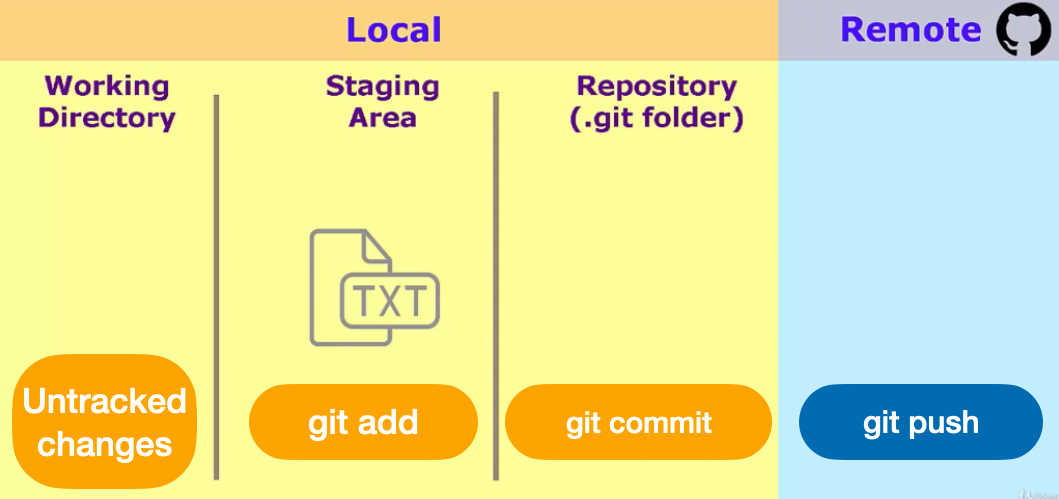
\includegraphics[width=0.5\textwidth]{images/git_stages.png}
				%				\vspace{-2mm}
				%				\captionof{figure}{Git states and associated commands. \href{https://www.udemy.com/course/git-complete/}{ \faLink{}  Source}}
				%			\end{minipage}
			
		\end{minipage}
	};
	\node[fancytitle, right=10pt, fill=outlinecolor, text=background, draw=outlinecolor, rounded corners] at (box.north west) {Commit History (2)};
\end{tikzpicture}
